\documentclass{elsarticle}
\usepackage{amssymb}
\usepackage{hyperref}
\usepackage{graphics}
\journal{Expert System with Applications}

\newtheorem{definition}{Definition}
\begin{document}

\begin{frontmatter}


\title{Knowledge Acquisition Method from Domain Text Based on Theme Logic Model and Artificial Neural Network \tnoteref{t1,t2}}
\tnotetext[t1]{This document is a collaborative effort.}
\tnotetext[t2]{The second title footnote.}

% use optional labels to link authors explicitly to addresses:
% \author[label1,label2]{}
% \address[label1]{}
% \address[label2]{}

\author[buaa]{Jun Wang\corref{cor1}}
\ead{king.wang@buaa.edu.cn}
\author[buaa]{Yunpeng Wu\corref{cor2}}
\ead{yunpeng.wu@sem.buaa.edu.cn}
\author[buaa]{Xuening Liu\corref{cor2}}
\ead{xx@gmail.com}


\cortext[cor1]{Corresponding author}
\cortext[cor2]{Principal corresponding author}
\fntext[fn1]{This is the specimen author footnote.}
\fntext[fn2]{Another author footnote, but a little more longer.}



\address[buaa]{School of Economics \& Management, Beihang University, Beijing 100083,
P.R. China }


\begin{abstract}
% Text of abstract
In order to acquire knowledge from domain text such as failure
analysis text of aviation product, a framework is proposed to enhance
the efficiency and accuracy of knowledge acquisition. In this
framework, sentence templates are defined to extract the
meta-knowledge and RDF is used to describe the extracted knowledge.
After the preprocessing steps, the authors propose a new model: theme logic
model (TLM) to present all the themes of a piece of text and the logical
relations among different themes. In this model, the text of each
theme can be represented as an attribute-value vector based on domain
ontology. Meanwhile, the logical relations are the domain knowledge to be
acquired. The theme logic model then will be transformed to the
training set of the artificial neural network to acquire the failure
analysis knowledge. After training process, acquired knowledge will be extracted by SD method from the artificial neural network and represented by rules. Therefore, a prototype is developed to acquire knowledge from failure analysis reports of aviation product. Empirical results show that the framework can acquire knowledge from domain text efficiently.
\end{abstract}

\begin{keyword}
% keywords here, in the form: keyword \sep keyword

% PACS codes here, in the form: \PACS code \sep code

% MSC codes here, in the form: \MSC code \sep code
% or \MSC[2008] code \sep code (2000 is the default)
Knowledge Acquisition; Domain Text; Theme Logic Model; Artificial Neural Network; Failure Analysis Report


\end{keyword}

\end{frontmatter}

\section{Introduction}
\label{sec:introduction}

Over the past decades, massive volumes of data have been collected in
corporations, of which more than eighty percent are stored in
text \cite{Mitchell2003}. Unfortunately, the explosive growth of
information has often resulted in frustrating situations when
corporations are not able to understand the knowledge it contains 
and organize the information well. Knowledge management is
implemented by enterprises and organizations to manage their knowledge
more effectively, including sorting useful knowledge from information, storing
knowledge in good order, and finding knowledge in an existing
knowledge base \cite{turban2001dss}. Knowledge acquisition from text
(KAT) , as an important way of knowledge acquisition, 
extracts useful knowledge from
text, especially domain text. And domain text is the text collection in a specific domain. Meanwhile, the domain texts here have two
main meanings: on one hand, the set of terms which are used to
describe their contents, and on the other, a well-defined structure to
organize these contents comprehensibly and improve readability for the
user \cite{Campos2004}. The text follows a certain controllable syntax
which can be easily summarized and formulated. Thus, the domain text
mentioned in this paper is semi-structured. 

The domain knowledge is valuable but often buried in domain texts
within a range of sources such as failure analysis reports of aviation
product, government files, records of meetings and experimental
reports, and so on. Mining domain text collection is useful for better understanding
the field. Through automated approaches, knowledge
associated to a specific domain can be extracted and integrated from
these disparate text sources. The acquired knowledge is valuable for a variety of applications including decision support, quality assurance and knowledge retrieval.

Many efforts have been devoted to automatic knowledge
acquisition from text \cite{salton1975vsm,361220,215383,Tai2002,130346} . The early knowledge acquisition systems focus mainly on indexing the
texts in the collection using Boolean model. Such model is over
simplified and cannot rank the relevant texts together with automatic
indexing. In this condition, Salton proposed Vector Space Model (VSM) in 1975 \cite{salton1975vsm,361220}. In this model, text is represented by vectors in a multidimensional space. To improve the performance of VSM, a number of enhanced methods have been put forward. Some based on dimensionality reduction and others using feedback information from the user \cite{Tai2002}. The former focuses on reducing the high-dimensional vector space into a low-dimensional one, among which the Latent Semantic Indexing (LSI) using Single Valued Decomposition is probably used most widely \cite{130346}. The latter uses feedback information from a user to increase the efficiency.

In this paper, the authors make great efforts to develop an effective methodology of
knowledge acquisition from domain text such as failure analysis
reports of aviation product based on a new text indexing model, theme
logic model. Salton described text themes as a main text decomposition
strategy \cite{234834}. The text theme is represented by semantically
homogeneous text pieces where all components treat a common subject
area. The theme logic model employs two sets to represent a text: a
set of themes in the text and a set of relations among the themes. The
text of each theme can be represented as an attribute-value vector
based on domain ontology, so the set of themes is a set of vectors of
all the themes in the text. In addition, there are meaningful logical
relations existing among different themes, and for a domain the logic
relation is the domain knowledge to be acquired. The theme logic model
then will be transformed to the training set of the artificial neural
network to acquire the failure analysis knowledge. We use  artificial
neural network since it is a learning-by-example paradigm in which
problem-solving knowledge is automatically generated according to
actual examples \cite{Huang2002,Kim2004}. Then the acquired knowledge  will be extracted by SD method from the artificial neural network and represented by rules \cite{130346,Sestito1991}. Furthermore, a prototype system is implemented and tested for scenario demonstration. Empirical results show that the framework can acquire knowledge from domain text efficiently.

This paper is organized as follows. In Section 2, we review some related work about knowledge acquisition from text and failure analysis. Then the framework of knowledge acquisition is explained in detail in Section 3. The structure analysis of domain text is presented in Section 4. Section 5 describes how to construct the theme logic model of domain text based on the domain ontology. And in Section 6, BP neural network is used to acquire the knowledge based on the theme logic model. Finally,  some experimental results are obtained and discussed in Section 7. Therefore, a conclusion is drawn in Section 8. 

\section{Related Work
}
\label{sec:related-work}

\subsection{Knowledge Acquisition from Text
}
\label{sec:knowl-acqu-from}

Knowledge acquisition from text is one of the most fruitful research
areas in artificial intelligence. Text-based knowledge acquisition
methods and tools can help to manage the wealth of information and
discover facts, relationships and implications in domain texts
\cite{Hahn2000,Gunn1999}. 

Gunn et al has discussed the existing knowledge acquisition techniques based
on manual learning, machine learning and logic programming \cite{Gunn1999}. The
manual learning methodology relies on knowledge engineers to acquire
and formalize knowledge from experts or free texts. However, since any
natural language is extremely difficult for computer systems to
understand, the machine learning and inductive logic programming
methodologies both require at least some manual processing of the
large quantity of source information
\cite{matwin:tac,Richardson1997}. Training set and background
knowledge must be built to aid and the interaction of knowledge
engineers is necessary. The result of an inductive system can never be
guaranteed to be accurate because identification of relevant features
and selection of representative examples are important to this
approach. None of the aforementioned KA techniques seems adequate for
acquiring knowledge from domain text, for the reasons given. 

Older knowledge acquisition systems operate on the principal of
indexing the texts in the collection. The most popular indexing
approach is based on the vector space model
\cite{361220,salton1975vsm} which is the most effective methodology \cite{215383}. In this model,
text is represented by vectors in an n-dimensional space, where n is
the number of distinct terms. There are three-step in this strategy where
terms are first extracted from the document text, then the weights of
the indexed terms are derived to improve the document retrieval
accuracy, and then the documents are ranked with respect to a
similarity measure \cite{Raghavan1986}. To improve the performance of
VSM, a number of enhanced methods have been proposed. The reduction of
the dimensionality of the model is one way to solve these
problems. The LSI model is accomplished by mapping a high-dimensional
space into a low-dimensional space by using SVD. Mao and Chu discuss three types of schemes, the stem-based, concept-based
and phrase-based schemes, showing the retrieval effectiveness of the
phrased-based VSM is significantly higher than that of the current
gold-standard—the term-based VSM \cite{Mao2007}. Wei et
al. brings forward an LSI-based multilingual document clustering technique
that employs LSI analysis to a parallel corpus and constructs a
multilingual semantic space, which reduces the dimensions and thereby
improves both clustering effectiveness and efficiency \cite{Wei2008}.

\subsection{Failure Analysis
}
\label{sec:failure-analysis-}

Failure, as defined by the International Electro-technical Commission
(IEC), is ‘the termination of the ability of an item to perform a
required function’. Whenever a failure occurs, the
failed component and the failure situation must be examined to
determine the cause. This investigation process is called failure
analysis \cite{Liao1999}. Robert suggests that there should be a
systematic way of performing failure analysis and the investigation
and analysis process will follow a logical series of stages
\cite{roberts1980stm}. An opinion regarding the failure mechanism will
be formed and a final conclusion will be reached by the domain
experts. Finally, a failure analysis will be written to note the
entire process of failure analysis. The failure analysis report is an
important source of engineering knowledge, which contains substantial
and essential failure knowledge and conveys some inherent phenomena or
regularities about the processes generating failure. Acquiring
knowledge from failure analysis report will lead to better designs,
material selections or fabrication modifications and important
economies \cite{Castro2004}. 

Traditionally, the failure analysis process is carried out by vast
numbers of human experts. However, as the volume of failure analysis
report is growing at explosive rate, this process becomes extremely
ineffective and inefficient. The availability and use of accurate
knowledge acquisition from this large volume is
required. Computer-assisted knowledge acquisition is necessary to
support quality decision-making and to overcome human cognitive
constraints.  Numerous studies have been conducted to develop
computer-assisted systems and various approaches have been taken such
as fault tree analysis \cite{Israel2006}, expert systems \cite{Kim2004}, neural
network \cite{Zakarian1999}, neuro-fuzzy system \cite{Chen2006}, etc. Mayer described an expert system for electric utility power plant personnel to identify a basic failure mechanism that can produce the type of boiler tube failure under investigation \cite{Mayer1990}. Liao developed an integrated database and expert system for identifying the failure mechanism of mechanical components \cite{liao1999ida}. Relatively fewer attempts have been made to develop computerized failure analysis systems in which knowledge is acquired from domain text such as failure analysis report.


\section{A Framework for Knowledge Acquisition from Domain Text
}
\label{sec:fram-knowl-acqu}

The aim of this framework is to acquire knowledge from semi-structured
domain texts. The knowledge acquisition is processed through several
modules including structure analysis, theme logic model construction
and artificial neural network, as shown in Figure 1. The structure
analysis transforms the failure analysis report into unique RDF by
defining sentence templates. The theme logic model represents all the
texts based on domain ontology using two sets: a set of all themes in
a text and a set of the relations among the themes. The frame-oriented ontology is a set of classes, relations, attributes and
values. The artificial neural network processes a training set which is 
transformed from the theme logic model based on the domain ontology,
and the acquired knowledge will be converted into knowledge rules. Finally, the acquired knowledge rules will be stored into a knowledge base.
\begin{figure}[htp]
  \centering
  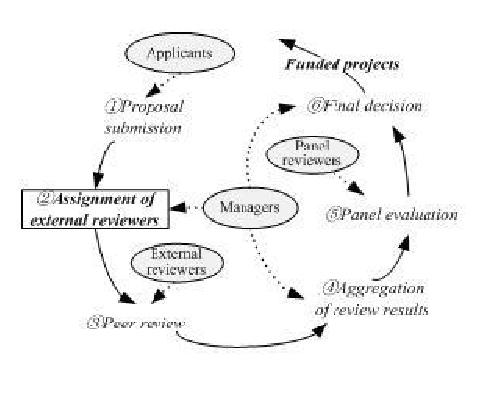
\includegraphics{esa/1.eps}

  \caption{The Framework for Knowledge Acquisition from Domain Text}
  \label{fig:1}
\end{figure}

\section{Structure Analysis of Domain Text 
}
\label{sec:struct-analys-doma}

There are tremendous domain texts in an enterprise, thus, the first step
is to transform them to a unique format. The main purpose of the
structure analysis and meta-knowledge acquisition is to analyze the
structure of the domain text and use meta-knowledge to help manage
them. As the base of OWL, RDF offers a generic framework and plays an
important role in the construction of semantic web \cite{lassila1999rdf}. Thus we
choose RDF and the output of the structure analysis is a set of RDF
documents, as is shown in Figure2. 
\begin{figure}[htp]
  \centering
  \includegraphics{esa/2.eps}

  \caption{Transform failure analysis report into RDF}
  \label{fig:2}
\end{figure}
Although written in natural language, the content of the domain text
is closely related to a specific domain and follows a certain
controllable syntax which can be easily summarized and
formulated. Thus the domain text mentioned in this paper is
semi-structured. And the main steps of transforming are in the following \cite{Wang2008}:
\begin{enumerate}
\item Analyze domain texts set (T-Set), and define a grammar G used for
defining the information extraction rule;
\item Define the information extraction rules set R;
\item Build a validator to test whether R conforms to the entire domain
texts;
\item If there are texts violate R, return to Step 3;
\item Write a parser to analyze the texts and find text blocks
matching rule in R, and transform T-Set to R-Set.  
\end{enumerate}


The purpose of structure analysis of domain text is to find the
modeling ways based on the structural characteristics of the domain
for further access to acquire knowledge and improve
the accuracy and efficiency of other follow-up
text-processing effectively. Salton has described two main text decomposition
strategies: a chronological decomposition into text segments
and semantic decomposition into text themes \cite{234834}. The text segment is
a contiguous piece of text units that are linked internally but
largely disconnected with the adjacent texts. The text theme is
represented by semantically homogeneous text pieces where all
components treat a common subject area.

As to the failure analysis report, it is usually in a certain format
in accordance with the requirements for writing. A well-defined structure is used to organize
the content comprehensibly and improve readability for the user. Thus,
the text segment and the text theme are easily found and
described. The text themes focus on the structure that contains the
text of the ideological content and logical way of expression. In this way, the segment and the theme of text is defined.

\begin{itshape}
  The text segment of failure analysis report= (title, author,
  abstract, chapter, section, paragraph, sentence). 

The text theme of failure analysis report= (title, author, abstract, phenomenon of the failure component, reasons and inference for the failure, judgment of the failure mode).

\end{itshape}

Different types of texts have different forms of
organization, and paragraph is a basic organizational
hierarchy. Different paragraphs constitute a hierarchy to express the
common theme in an orderly manner. The division of text theme is based
on the common subjects expressed by several paragraphs. And logic
relations often exist among different themes of a text. As to
failure analysis report, ' phenomenon of the failure component’, ‘reasons and inference of failure’, ‘judgment of failure mode’ constitute three themes and there are meaningful logic relations among them. Failure analysis report is a form record of the entire failure analysis process, in which the domain experts use the failure analysis techniques to do experiment, observe and analyze the failure phenomena to determine the causes of failure and make the necessary preventive measures based on their own knowledge in a particular field \cite{roberts1980stm}. Therefore, the logic relation between the themes ‘phenomenon of the failure component’ and ‘judgment of failure mode’ is the essential logic mapping from failure phenomenon to failure mode, which is the very failure knowledge to be acquired. Consequently, a new theme logic model to express the logic relation between different themes is built.



\begin{definition}
  The theme logic model of a text with n different themes is :
\[ d = (T = \{T_1,T_2,\ldots,T_n\}, R = \{R_{ij} = R(T_i,T_j) \, | \, T_i,T_j \in
T,1\le i,j \le n \}) \]
where $T$ represents a set of themes in the text, $R$ represents a set of logic relation between two themes, $R_{ij}$ represents the logic relation between themes $T_i$ and $T_j$. 

\end{definition}

\section{Theme Logic Model of Dom
}
\label{sec:theme-logic-model}

In order to acquire the domain knowledge of failure analysis, we
choose two themes: ‘Phenomenon of the failure component’ (represented
by $P$) and ‘judgment of failure Mode’ (represented by $M$) to construct
the theme logic model of failure analysis report as $d = (T = \{P,M\},
R = \{R_{PM}\})$.

$R_{PM}$ ,representing the logic relations between theme $P$ and $M$, is the domain knowledge to be acquired. In failure analysis, the
domain experts use their tacit knowledge to connect various phenomena
with a specific failure mode, but the tacit knowledge in their minds is
not easily to be expressed and transformed to explicit knowledge even
by the domain experts themselves. As a result, the
knowledge acquisition becomes a bottleneck in knowledge
engineering. In view of this, the authors of this paper intend to construct a theme logic model of the domain
texts and transform them into the training set of artificial neural
network to acquire knowledge. More precisely, the text in each
theme will be represented with an attribute-value vector based on the
domain ontology. 

The failure analysis techniques used by domain experts are relatively
fixed, such as trace analysis, crack analysis and fracture
analysis. Each analysis techniques observes phenomena of failure
components from different perspectives. And the observed phenomena and
the attributes of each phenomenon can be clearly described by domain
ontology. In addition, the language and sentence structure used to express and describe the failure phenomena are usually relatively fixed. Therefore, the text of each theme can be presented by an attribute-value vector in an n-dimensional space based on lightweight domain ontology of failure analysis, which is frame-oriented and a set of classes, relations, attributes and values \cite{747902}.

\begin{definition}
  The attribute-value vector of theme $T_i$ in text is defined as:
\[AVV_i = \{<a_1,v_1>,<a_2,v_2> \ldots,<a_n,v_n>\} \]
\end{definition}
$a_i$ represent the attributes in theme $T_i$, and $v_i$ represents the value of attribute $a_i$ , $n$ is the number of distinct attributes in domain ontology.

\begin{definition}
  A lightweight domain ontology ($O$) models a specific domain, and is
  made up of a set of Concepts ($C$), Attributes ($A$), Attribute
  Value ($V$) and Relations between the Concepts ($R$):$O = \{C,A,V,R\}$


\end{definition}

Concepts (or classes) are the abstract nodes or collections of objects. Attributes provide extra features and are used to identify and describe the concept. Each attribute has at least a name and a value, and is used to store information that is specific to the object it is attached to. In addition, the value of an attribute can be a complex data type, such as a numerical interval or a set. Relation is used to indicate a similarity between two concepts within ontology. The four elements are shown in Figure 3.
\begin{figure}[htb]
  \centering
  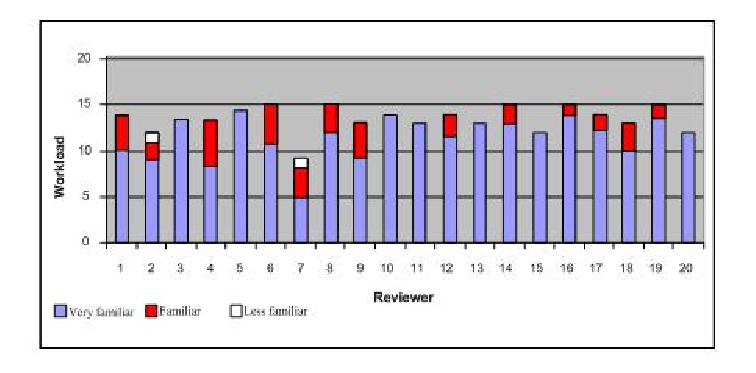
\includegraphics{esa/3.eps}
  \caption{Elements in Lightweight Domain Ontology}
\end{figure}
There are three steps to construct attribute-value vector.
\begin{enumerate}
\item Pretreatment. For the text of each theme in RDF documents to be processed, all the standing alone punctuation marks are removed first and the text will be divided into sections by full stop and comma.
\item  Construct lightweight domain ontology. The lightweight domain ontology comprises two sub-ontologies: failure analysis technique ontology and failure mode ontology. Ontology construction is a large and tedious task. But here we only need lightweight domain ontology to express all the concepts, relations, attributes and values. Thus, it is much easier to construct it. Moreover, a synonym base will be also included to store all the words having the same or nearly the same meaning as the attribute and attribute value in a language. 
\item Extract attribute-value vector based on lightweight domain ontology.

\end{enumerate}

We do word segmentation and use string matching to identify and collect the attributes and values based on the lightweight domain ontology. The similarity of attribute (or attribute value) S1 of string S2 is defined as follows.
\begin{definition}
  Similarity of Attribute (or Value) S1 of String
  S2 \[similarity(S_1,S_2) = \frac{V(S_1) \cap V(S_2)}{V(S_1)} \]

\end{definition}

$V(S_1)$ represents the number of single words in $S_1$, and $V(S_1)
\cap V(S_2)$ represents the common single words in $S_1$ and $S_2$.

The algorithm to construct attribute-value vector is as follows. ‘a’ and ‘b’ are two indicators of similarity.

\begin{verbatim}
Input: 
A theme in RDF
Lightweight domain ontology 
String[] GetSynonymy (String) //a function to get the synonym of a word

Output:
attribute-value vector of a theme

Algorithm:
Each sentence in the theme is divided into sub sections by full stop and comma to form a vector of sub sentence vector={C1,C2,…,Ci,…,Cn} 

For each Ci, i=1,2,..n 
For each ai of Ontology 
aSyn=GetSynonymy(ai)
    Foreach s of aSyn
	  Search s in Ci

       IF similarity>a THEN
		 For each vi,j of ai
  			vSyn=GetSynonymy(ai)
    			 For each c of vSyn
				Search c in Ci
        			IF similarity> THEN
				Add < ti, vi,j> to attribute-value vector
			    ELSE Next c
  ELSE Next s

\end{verbatim}

\section{Knowledge Acquisition Based on Theme Logic Model and Artificial Neural Network}
\label{sec:knowl-acqu-based}

Artificial neural network belongs to the family of learning-by-example
paradigm in which problem-solving knowledge is automatically generated
according to actual examples \cite{hassoun1995fan}. As there is a very
complicated nonlinear relation between the phenomena of failure and
the failure mode, it is difficult to establish a suitable model in
practice. Whereas, Artificial neural network with its adaptive, self-learning
and non-linear system of powerful analytical capacity provides a new
solution for failure analysis. The main steps are in the following:
\begin{enumerate}
\item Design the architecture of artificial neural network.
\item Transform the theme logic model into the training set of the
  neural network, train and test the neural network. 
\item  Extract knowledge from neural network and represent the
knowledge with rules.
\end{enumerate}


\subsection{Artificial Neural Network Design}
\label{sec:artif-neur-netw}

The ANN can be classified into several categories based on supervised
and un-supervised learning methods and feed-forward and feedback
recall architectures. The back-propagation network algorithm (BPNN) is
a multi-layered network first proposed by Rumelhart
\cite{rumelhart1986lir}. The algorithm is also called a supervised
learning method that can be used to solve non-linear problems. The
learning stage of BPNN involves a forward pass and a backward pass. An
advantage of BPNN is that it does not need to change the network
structure or activation functions of nodes and only adjusts the
weights between nodes in the network \cite{Massey2003}. BPNN is one of the most
frequently utilized neural network techniques for classification and
prediction \cite{graupe2007pan}. In this paper, the authors also use the
BPNN architecture in a supervised learning method to acquire knowledge
from domain text. The neural network is concerned with acquiring
failure knowledge from a set of data consisting of the theme logic
model. 

BPNN architecture comprises of an input layers, an output layer and hidden layers. The BPNN parameters include a number of hidden layers, a number of hidden neurons, an activation function, learning rate, momentum, etc. All of these have significant impact on the performance of BPNN.
\begin{itemize}
\item The input neurons are used to represent the phenomena of failure
  component for each attribute-value vector, which is according to the attribute value of failure analysis technique ontology.
\item The output neurons are used to reflect the failure mode of failure component. There are different hierarchies of failure mode. We can assign the output neurons to reflect a specific hierarchy of failure mode and the knowledge mapping the phenomena to this hierarchy of failure mode will be acquired. 
\item One hidden layer is sufficient for computing arbitrary decision
  boundaries for the output in most cases \cite{Khaw1995}. It is important to
  mention that there is no standard formula for calculating the number
  of nodes in the hidden layer \cite{turban:oaj}. Maren, Harston
  and Pap demonstrated that the bound of neurons in the hidden layer
  was between $2N_i+1$ and $N_o(N_i +1)$, where $N_i$ is the number of
  input nodes and $N_o$ is the number of output nodes
  \cite{maren1990hnc}. The number of hidden nodes are selected through
  experiment between $2N_i+1$ and $N_o(N_i +1)$. 
\item The activation function is mathematical formula that determines the output of a processing neuron. Logistic activation functions are employers in the hidden layer and linear activation is utilized in the output layer.  
\item As to the learning rate and momentum, most ANN software package provides default values for both parameters that typically work well. The learning rate determines the speed at which the weight changes and the momentum constant prevents sudden changes in attaining the results.  


\end{itemize}

\subsection{Transform the Theme Logic Model to Training Set}
\label{sec:transf-theme-logic}

Every training sample is represented by theme logic model, and then
every theme in the mode will be represented by an attribute-value
vector as the training data of the BPNN. The $P$ theme will be  used as
the input vector of the BPNN while the $M$ theme as the output vector of
the BPNN. Each attribute value in ontology will be included in the
input vector or output vector. For each transformed result, if the attribute value exist in it, assign the attribute value to 1 in the input vector else to 0. 

After transformation, a set of n-dimensional input vectors are obtained. Under  such condition, put the entire input vectors transformed from m sample texts together to form the input matrix. 

\[
Input - Matrix = \bordermatrix{%
& V_1 & V_2 & \cdots & V_j & \cdots & V_n \cr
& v_{11} & v_{12} & \cdots & v_{1j} &  \cdots & v_{1n} \cr
& v_{21} & v_{22} & \cdots & v_{2j} &   \cdots & v_{2n} \cr
& \vdots & \vdots & \ddots  \cr
& v_{i1} & v_{i2} & \cdots & v_{ij} & \cdots & v_{in} \cr
& \vdots & \vdots & &  & \ddots  \cr
& v_{m1} & v_{m2} & \cdots & v_{mj} & \cdots & v_{mn} \cr
}
\]

In order to enhance the efficiency of BPNN, a threshold k is defined to
reduce the dimension of input vector by removing the input nodes whose k
value is more than a threshold. For a specific attribute value $v_j$,
$k_j$ is defined as follows. 
\[k_j = \frac{\sum_{i=1}^{m}no.of.zero(v_{ij})}{m}\]

In fact, a higher k value of a specific attribute value indicates a lower importance in identifying the failure mode. In experiment, k can be assigned different values to reduce the dimension of input vector and find the best k value for BPNN.

After determining the best k value, the BPNN can be trained and tested by samples. The precision rate is the indicators for evaluating the BPNN’s performance, which measures the percentage of  the right prediction of the test samples. 

\subsection{Knowledge Extract from Artificial Neural Network }
\label{sec:knowl-extr-from}

Neural network generally represent knowledge at the lower level, while
knowledge based systems use higher level knowledge
representations. The knowledge acquired by neural network needs to be
extracted and represented in the forms of rules, frames or semantic
nets. Sestito and Dillion proposed a SD method to extract knowledge
from neural network \cite{Sestito1991,130346}. The main steps include:

\begin{enumerate}
\item Extend the input nodes to include all the output nodes and
  training the new network with Back-propagation.
\item Compute the Sum of Squared Error (SSEab) to measure the contribution of input a to output b.
\[SSE_{ab} = \sum_{j=0}^{no.of.hidden.units}{(w_{bj}-w_{aj})}^2\]

$no.of.hidden.units$represents the number of hidden nodes,
$w_{aj}$represents the value of the link between input $a$ and hidden
node $j$, $w_{bj}$ represents the value of the link between output $b$
and hidden node $j$. 
\item  Negate the input attributes while keeping the output attributes
constant and use the Hebb’s rule to determine the inhibition links
$weight_{ab}$ between the input $a$ and the output $b$.
\item Compute the product between $SSE_{ab}$ and
$weight_{ab}$. $Product_{ab}$ indicates which input is associated with
an output. These $Product_{ab}$ will be closed to or equivalent to
zero for those attributes which are directly associated. Thus, the
input attributes using a particular output which have a small or zero
product are taken to the attributes defining the output. These input
attributes are taken to be part of the antecedent and the output is
taken to be the consequence of a rule. 

\[Product_{ab} = SSE_{ab}\times weight_{ab}\]

\end{enumerate}

\section{Experiments and Discussions }
\label{sec:exper-disc-}

\subsection{Experiments Design
}
\label{sec:experiments-design-}

In order to measure the performance of the framework, we develop a
prototype  to acquire domain
knowledge from 400 failure analysis reports of aviation engine. All
the reports were divided into two groups: 300 documents are used for
training and 100 documents are used for testing. The reports are
related to four kinds of fracture failure, namely brittle fracture,
overload fracture, fatigue fracture, environment fracture
\cite{medema}.

The BPNN’s development and training followed the algorithm analyzed in
the previous sections using MATLAB 7 application tool. There
are four output nodes according to four kind of fracture failure and
the number of input node is determined by $k$. The maximum number of
epoch for the BPNN was set as 2000 and the error goal was 0.001. As
there are not formula to compute the number of nodes in hidden layer,
it was selected through experiment around between $2Ni+1$ and $N_o(N_i
+1)$. The BPNN used ‘traingdx’ as learning algorithm. Other parameters
used default. The architecture of BPNN is shown in Figure 4.
\begin{figure}[htb]
  \centering
  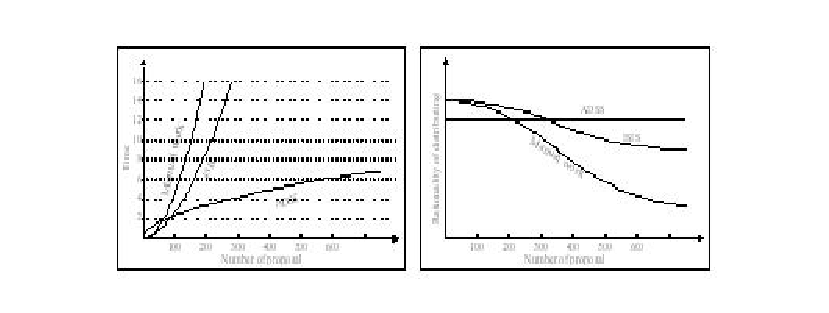
\includegraphics{esa/4.eps}
  \caption{Architecture of the BPNN for Knowledge Acquisition
  }
\label{fig:4}
\end{figure}

\subsection{Results and Analysis
}
\label{sec:results-analysis-}

The attribute-value vector of the $P$ theme is extracted by the prototype system as is shown in Figure 5.

 \begin{figure}[htb]
  \centering
  \scalebox{0.38}{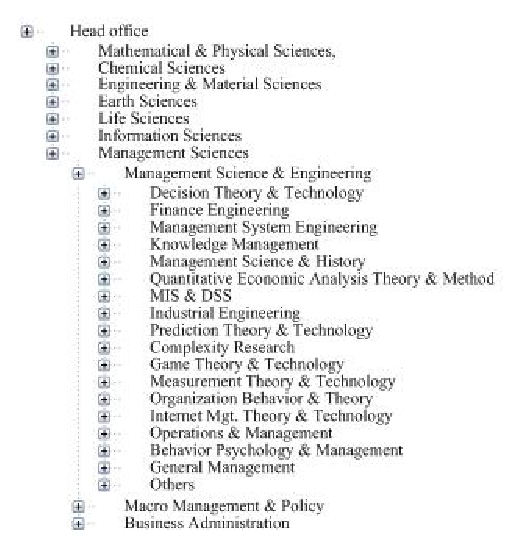
\includegraphics{esa/5.eps}}
  \caption{Theme logic model of training samples}
\label{fig:5}
\end{figure}

The neural network’s input nodes number is equal to the number of column in the input matrix, corresponding to the number of attribute value in domain ontology of failure analysis technique. There are 68 distinct attribute values for fracture failure. We remove the columns in the input matrix whose value is all zero, and 41 distinct attribute values remain. That means the number of inputs nodes ranges from 1 to 41. We assign 1, 0.95, 0.9, 0.85, 0.8, 0.75, 0.7 to k and choose five different number of hidden nodes between $2N_i+1$ and $N_o(N_i +1)$ to design different BPNN. And the result is shown in Figure 6.

 \begin{figure}[htb]
  \centering
  \scalebox{0.33}{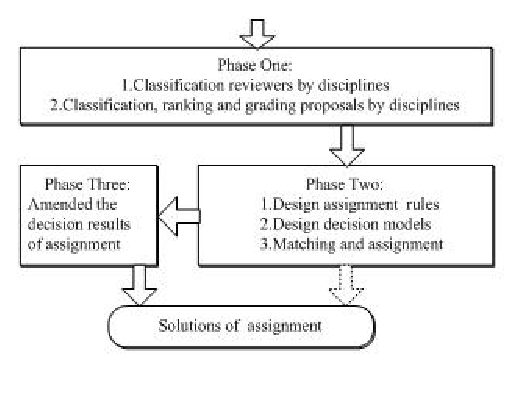
\includegraphics{esa/6.eps}}
  \caption{Experiment results of different $k$ value}
\label{fig:6}
\end{figure}
 
Out of all the networks tested, a network with $k$ is equal to 0.8 and 56
hidden nodes reached the best performance goal when compared with
other networks. Then $Product_{ab}$  was computed to indicate the
association of a specific input node to an output node, namely the
association of a specific failure phenomenon to a failure mode as is
shown in Figure 7. 

 \begin{figure}[htb]
  \centering
  \scalebox{0.33}{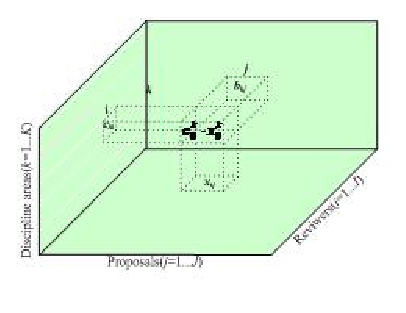
\includegraphics{esa/7.eps}}
  \caption{The association of failure phenomenon to failure mode measured by $Product_{ab}$
}
\label{fig:7}
\end{figure}

For each output node $b$, sort all of its corresponding $Product_{ab}$
descend and select the appropriate cut-off points. The selection of
cut-off point should be based on the SD method and the characteristics
of the domain. The input below cut-off point will be grouped together
in the antecedent and the output is taken to be the consequent of the
rule. Take the first output as an example, the following rule will be
extracted:
\begin{verbatim}

(IF       ‘Surface morphology’=‘Pit’ 
AND  ‘Defects in materials presented by fracture’=‘Yes’
AND  ‘Tendency of fracture or crack’=‘Along crystal expansion’
AND  ‘Trace type’=‘Trace of mechanical contacts’, ‘Manufacturing trace’
THEN   ‘Failure mode’=‘Brittle fracture’
)

\end{verbatim}

\section{Conclusion and Future Research 
}
\label{sec:concl-future-rese}

Extracting knowledge from semi-constructured is an indispensable while
complicated task for knowledge organization. In this paper, the authors
propose a framework for knowledge acquisition from domain text
based on theme logic model and artificial neural network to acquire knowledge from
failure analysis reports. And the  performance is evaluated. Experiments show the framework is relatively
easy to use and can extract meaningful knowledge effectively. 
Knowledge acquisition from domain text is a process of comprehensive
analysis and incremental improvement. In the future, more experiments are
needed to carry out to testify the capability of this framework. And
it should be extended to improve the domain ontology to enhance the
efficiency of theme logic model generation.

\section{Acknowledgment}
\label{sec:acknowledgment}

The work described in this paper was fully supported by a grant from ***( Project No.  ). 



\bibliographystyle{elsarticle-num}
\bibliography{../../bibtex/elsevier,../../bibtex/emerald,../../bibtex/chinese,../../bibtex/jstor,../../bibtex/citeseer,../../bibtex/acm,../../bibtex/wiley,../../bibtex/book,../../bibtex/thesis,../../bibtex/ebsco,../../bibtex/old,../../bibtex/ieee.bib,../../bibtex/springer,../../bibtex/internet,../../bibtex/worldacademic}

\end{document}

